\documentclass[11pt,letterpaper,titlepage]{article}

\usepackage{geometry}
\geometry{left=2cm,right=2cm,top=2cm,bottom=3cm}

\usepackage{setspace}
\onehalfspacing

\usepackage{booktabs}

\usepackage{tikz}

\usetikzlibrary{automata, positioning, arrows}

\newcounter{wavenum}

\setlength{\unitlength}{0.1cm}
% advance clock one cycle, not to be called directly
\newcommand*{\clki}{
  \draw (t_cur) -- ++(0,.3) -- ++(.5,0) -- ++(0,-.6) -- ++(.5,0) -- ++(0,.3)
    node[time] (t_cur) {};
}

\newcommand*{\bitvector}[3]{
  \draw[fill=#3] (t_cur) -- ++( .1, .3) -- ++(#2-.2,0) -- ++(.1, -.3)
                         -- ++(-.1,-.3) -- ++(.2-#2,0) -- cycle;
  \path (t_cur) -- node[anchor=mid] {#1} ++(#2,0) node[time] (t_cur) {};
}

% \known{val}{length}
\newcommand*{\known}[2]{
    \bitvector{#1}{#2}{white}
}

% \unknown{length}
\newcommand*{\unknown}[2][XXX]{
    \bitvector{#1}{#2}{black!20}
}

% \bit{1 or 0}{length}
\newcommand*{\bit}[2]{
  \draw (t_cur) -- ++(0,0.6*#1) -- ++(#2,0) -- ++(0,-0.6*#1)
    node[time] (t_cur) {};
}

% \unknownbit{length}
\newcommand*{\unknownbit}[1]{
  \draw[ultra thick,black!50] (t_cur) -- ++(#1,0) node[time] (t_cur) {};
}

% \nextwave{name}
\newcommand{\nextwave}[1]{
  \path (0,\value{wavenum}) node[left] {#1} node[time] (t_cur) {};
  \addtocounter{wavenum}{-1}
}

% \clk{name}{period}
\newcommand{\clk}[2]{
    \nextwave{#1}
    \FPeval{\res}{(\wavewidth+1)/#2}
    \FPeval{\reshalf}{#2/2}
    \foreach \t in {1,2,...,\res}{
        \bit{\reshalf}{1}
        \bit{\reshalf}{0}
    }
}

% \begin{wave}[clkname]{num_waves}{clock_cycles}
\newenvironment{wave}[3][time]{
  \begin{tikzpicture}[draw=black, yscale=.7,xscale=1]
    \tikzstyle{time}=[coordinate]
    \setlength{\unitlength}{0.5cm}
    \def\wavewidth{#3}
    \setcounter{wavenum}{0}
    \nextwave{#1}
    \foreach \t in {0,1,...,\wavewidth}{
      \draw[dotted] (t_cur) +(0,.5) node[above] {\t} -- ++(0,.4-#2);
      \clki
    }
}{\end{tikzpicture}}

\usepackage{graphicx}

\usepackage{listings}

\lstdefinestyle{mystyle}
{
    basicstyle=\small\ttfamily,
    % numbers=left,
    numbersep=11pt,
    tabsize=4,
    moredelim=*[s][\colorIndex]{[}{]},
    literate=*{:}{:}1
}

\lstset{style=mystyle}

\usepackage{fancyhdr}

\pagestyle{fancy}
\lhead{}
\rhead{}
\lfoot{ECEN 749 Section 601 Assignment 3}
\cfoot{\thepage}
\rfoot{@Lei Wang (Wilson)}
\renewcommand{\headrulewidth}{0pt}
\renewcommand{\headwidth}{\textwidth}
\renewcommand{\footrulewidth}{0.4pt}
\newcommand{\RomanNumeralCaps}[1]
{\MakeUppercase{\romannumeral #1}}

\begin{document}

\begin{enumerate}
    
    \item %Q1
    
    \begin{enumerate}
        
        \item %a
        
        $OUT = IN1 \cdot \overline{IN2} \cdot IN3 + \overline{IN1} \cdot IN2 \cdot IN3$
        
        The truth table is:
        
        \begin{table}[ht]
        \centering
        \begin{tabular}{@{}cccc@{}}
        \toprule
        IN1 & IN2 & IN3 & OUT \\ \midrule
        0   & 0   & 0   & 0   \\ \midrule
        0   & 0   & 1   & 0   \\ \midrule
        0   & 1   & 0   & 0   \\ \midrule
        0   & 1   & 1   & 1   \\ \midrule
        1   & 0   & 0   & 0   \\ \midrule
        1   & 0   & 1   & 1   \\ \midrule
        1   & 1   & 0   & 0   \\ \midrule
        1   & 1   & 1   & 0   \\ \bottomrule
        \end{tabular}
        \end{table}
        
        \begin{figure}[ht]
            \centering
            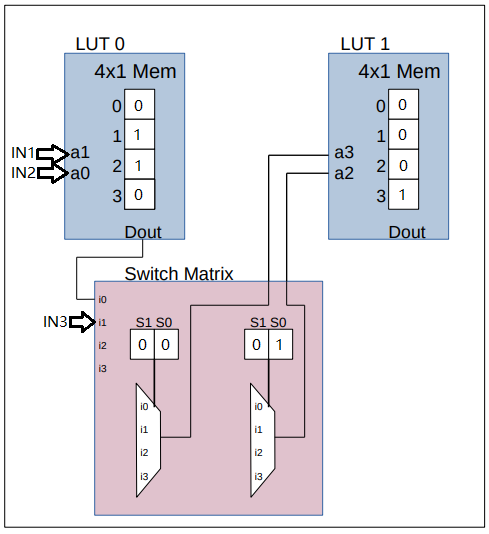
\includegraphics[width=0.5\textwidth]{Q1a.PNG}
            \caption{Q1)a}
        \end{figure}
        
        \newpage
        
        \item %b
        
        Bitstream will be 011000010001. Using the programming chain in Figure 2. The programming chain starts from the top left.
        
        \begin{figure}[ht]
            \centering
            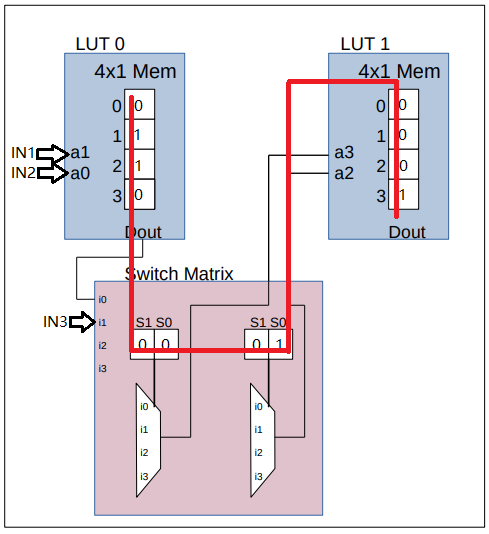
\includegraphics[width=0.5\textwidth]{Q1b.PNG}
            \caption{Q1)a}
        \end{figure}
        
    \end{enumerate}
    
    \item %Q2
    
    \begin{enumerate}
        
        \item %a
        
        Path 1, shown in Figure 3, with delay $5+3+3+3=14$ ps.
        
        \begin{figure}[ht]
            \centering
            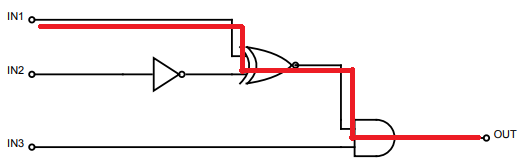
\includegraphics[width=0.6\textwidth]{path1.PNG}
            \caption{Q2)a}
        \end{figure}
        
        \newpage
        
        Path 2, shown in Figure 4, with delay $1+2+5+3+3+3=17$ ps.
        
        \begin{figure}[ht]
            \centering
            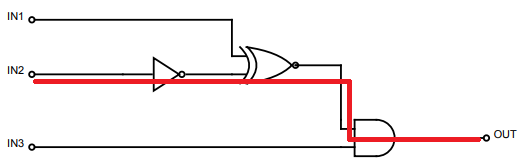
\includegraphics[width=0.6\textwidth]{path2.PNG}
            \caption{Q2)a}
        \end{figure}
        
        Path 3, shown in Figure 5, with delay $3+3=6$ ps.
        
        \begin{figure}[ht]
            \centering
            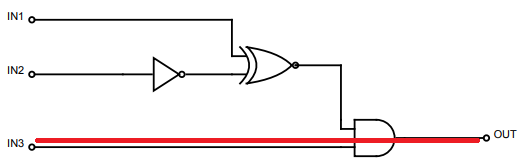
\includegraphics[width=0.6\textwidth]{path3.PNG}
            \caption{Q2)a}
        \end{figure}
        
        Overall, the worst case delay through the circuit is 17 ps.
        
        \item %b
        
        Adding the delay from the input to the register and the delay from the output to the register, the worst case delay is 22 ps. The highest clock frequency this circuit can achieve is 45.45 MHz.
        
    \end{enumerate}
    
    \item %Q3
    
    The fastest path is the following, with delay 6 ps.
    
    \begin{figure}[ht]
        \centering
        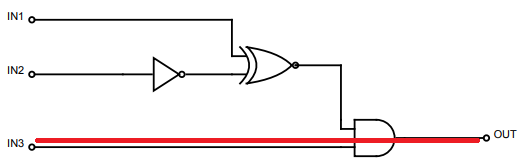
\includegraphics[width=0.6\textwidth]{path3.PNG}
        \caption{Q3}
    \end{figure}
    
     A "too fast" circuit may cause the circuit to violate timing constraint. A latch that does not have enough time to hold the signal may output signal that is random: only the signal output after the hold time is usable. Clock skew or jitter results in delay when synchronizing different components of the circuits. Some components that receive the clock signal earlier may carry out functions earlier than those that receive the clock signal later. If such circuits are time critical, i.e. depend on precise timing between different stages of the workflow, the circuit may use some random signal instead of the correctly propagated signal from an earlier stage and causes error.
    
\end{enumerate}

\end{document}
